\documentclass[12pt,a4paper]{article}
\usepackage[utf8]{inputenc}
\usepackage[T1]{fontenc}
\usepackage[french]{babel}
\frenchsetup{StandardItemLabels=true}
\usepackage{mathptmx}
\usepackage[a4paper,left=2.4cm,right=2.4cm,top=2.6cm,bottom=2.6cm,headheight=15pt]{geometry}
\usepackage{graphicx}
\usepackage[table]{xcolor}
\usepackage{array,tabularx,booktabs}
\usepackage{titlesec}
\usepackage{fancyhdr}
\usepackage{enumitem}
\usepackage{caption}
\renewcommand\tabularxcolumn[1]{m{#1}}
\usepackage{tocloft}
\usepackage[hidelinks]{hyperref}

\definecolor{bleu}{HTML}{15569E}
\definecolor{bleuclair}{HTML}{7FB3E6}
\definecolor{gris}{HTML}{5C6268}

\graphicspath{{img/}}
\setlength{\parindent}{0pt}
\setlength{\parskip}{6pt}
\linespread{1.15}

\titleformat{\section}{\normalfont\Large\bfseries\color{bleu}}{\thesection.}{0.6em}{}
\titleformat{\subsection}{\normalfont\large\bfseries\color{bleu}}{\thesubsection.}{0.6em}{}
\titlespacing*{\section}{0pt}{18pt}{8pt}
\titlespacing*{\subsection}{0pt}{12pt}{6pt}
\renewcommand{\cfttoctitlefont}{\Large\bfseries\color{bleu}}
\renewcommand{\cftsecfont}{\bfseries}
\renewcommand{\cftsecleader}{\cftdotfill{\cftdotsep}}

\pagestyle{fancy}
\fancyhf{}
\fancyhead[L]{\small\color{gris}IG-GIMAC-01 v1.0}
\fancyhead[R]{\small\color{gris}Moabi, module de certification}
\fancyfoot[L]{\small\color{gris}GIMAC}
\fancyfoot[C]{\small\color{gris}Présentation des interfaces}
\fancyfoot[R]{\small\bfseries\color{bleu}\thepage}
\renewcommand{\headrulewidth}{0.4pt}
\renewcommand{\footrulewidth}{0.4pt}

\captionsetup{labelfont={bf,color=bleu},font=small,justification=centering,labelsep=period}

% Capture d'écran suivie de son explication, sans coupure de page entre les deux.
\newcommand{\ecran}[3]{%
  \par\noindent\begin{minipage}{\linewidth}
  \centering\setlength{\fboxsep}{0pt}\fcolorbox{gris!40}{white}{\includegraphics[width=0.86\linewidth]{#1}}
  \captionof{figure}{#2}
  \vspace{2pt}
  {\leftskip=0pt\rightskip=0pt\parfillskip=0pt plus 1fil\relax #3\par}
  \end{minipage}\par\vspace{14pt}}
\newcommand{\justifying}{\rightskip=0pt plus 0pt\spaceskip=0pt\xspaceskip=0pt\relax}

% Pastille de couleur de la charte.
\newcommand{\pastille}[1]{\definecolor{pastilletmp}{HTML}{#1}\fcolorbox{gris!50}{pastilletmp}{\rule{0pt}{14pt}\rule{34pt}{0pt}}}

\begin{document}

% ------------------------------------------------------------------ Page de garde
\begin{titlepage}
\thispagestyle{empty}
\centering
\vspace*{-0.8cm}

\includegraphics[height=1.6cm]{gimac-logo-couleur.png}\par
\vspace{0.5cm}
{\bfseries GROUPEMENT INTERBANCAIRE MONÉTIQUE DE L'AFRIQUE CENTRALE}\par
\vspace{0.2cm}
{\small Banque des États de l'Afrique Centrale (BEAC)}\par
{\small Département Exploitation et Supervision (DES)}\par
\vspace{0.5cm}
{\color{bleu}\rule{\linewidth}{1.6pt}}\par
\vspace{0.6cm}
{\fontsize{24}{31}\selectfont\color{bleu}PRÉSENTATION DES INTERFACES\\ DU MODULE DE CERTIFICATION\par}
\vspace{0.5cm}
{\large\bfseries\color{gris}MOABI, PLATEFORME DE SUIVI DES ACTIVITÉS DU DES}\par
\vspace{0.4cm}
{\itshape Écrans, fenêtres de dialogue et charte graphique du parcours de certification\\ des liaisons des participants au réseau monétique}\par
\vspace{0.45cm}
{\color{bleuclair}\rule{\linewidth}{0.8pt}}\par
\vspace{0.45cm}
\renewcommand{\arraystretch}{1.1}\begin{tabular}{>{\raggedleft\bfseries}p{4.6cm} p{9.2cm}}
Référence & \textbf{IG-GIMAC-01 v1.0}\\[0pt]
Statut & \textbf{Document de présentation}\\[0pt]
Nature & Présentation commentée des interfaces graphiques\\[0pt]
Périmètre & Module de certification (étapes 1 à 10 du parcours)\\[0pt]
Documents amont & CC-GIMAC-01 v1.1, DS-GIMAC-01 v1.2, REC-GIMAC-01\\[0pt]
Établi par & \textbf{KOAGNE ISSA RYAN}, Ingénieur en Informatique et Systèmes d'Information\\[4pt]
Sous la supervision de & \textbf{Mme EKOUTOU GUILEINE}\\
 & \textbf{M. TABANGOLI Anthony}\\
 & \textbf{M. SOSSY Martial}\\
\end{tabular}
\vfill
{\color{gris}GIMAC, Siège Social, Yaoundé, République du Cameroun\\
Plateforme de suivi des activités du DES\\
Octobre 2026}
\end{titlepage}

% ------------------------------------------------------------------ Fiche d'identification
\section*{Fiche d'identification du document}
\renewcommand{\arraystretch}{1.5}
\begin{tabularx}{\linewidth}{|>{\bfseries\color{bleu}}m{4.2cm}|X|}
\hline
\rowcolor{bleu}\multicolumn{2}{|c|}{\textcolor{white}{\textbf{Informations générales}}}\\ \hline
Titre & Présentation des interfaces du module de certification\\ \hline
Référence & IG-GIMAC-01 v1.0\\ \hline
Version & Version 1.0 (première diffusion)\\ \hline
Date d'émission & 1er octobre 2026\\ \hline
Établi par & KOAGNE ISSA RYAN, Ingénieur en Informatique et Systèmes d'Information\\ \hline
Organisme & Groupement Interbancaire Monétique de l'Afrique Centrale (GIMAC)\\ \hline
Direction métier & Département Exploitation et Supervision (DES)\\ \hline
Destinataires & Collaborateurs du GIMAC associés au parcours de certification : DES, DDRM, Normes et Agréments, pôles réseau et système, production monétique, sécurité des systèmes d'information, conformité, direction générale\\ \hline
Objet & Montrer chaque écran et chaque fenêtre de dialogue du module, avec une explication simple, ainsi que la charte graphique\\ \hline
\end{tabularx}

\vspace{1cm}
\section*{Historique des versions}
\begin{tabularx}{\linewidth}{|c|c|m{3.6cm}|X|}
\hline
\rowcolor{bleu}\textcolor{white}{\textbf{Version}} & \textcolor{white}{\textbf{Date}} & \textcolor{white}{\textbf{Auteur}} & \textcolor{white}{\textbf{Description}}\\ \hline
v1.0 & 01/10/2026 & KOAGNE ISSA RYAN & Première version : préambule sur le nom Moabi, charte graphique, écrans et fenêtres de dialogue du module de certification.\\ \hline
\end{tabularx}
\clearpage

\tableofcontents
\clearpage

% ------------------------------------------------------------------ 1. Introduction
\section{Introduction}
Le GIMAC met en place une plateforme pour suivre les activités du Département Exploitation et Supervision. Son premier module couvre la certification : c'est le chemin que suit une institution, de la prise de contact jusqu'à la mise en production de sa liaison au réseau monétique, puis le suivi qui vient après.

Ce document présente les écrans de ce module, tels qu'ils apparaissent aujourd'hui. Il s'adresse aux collaborateurs du GIMAC qui vont utiliser la plateforme ou valider son contenu. Chaque capture d'écran est suivie d'une courte explication : ce que l'on voit, à qui l'écran est destiné et ce qu'on peut y faire.

Le document s'ouvre sur le choix du nom de la plateforme, Moabi. Vient ensuite la charte graphique : logo, couleurs, polices, motifs et éléments d'interface. Les écrans sont ensuite présentés dans l'ordre du parcours et par acteur : l'accès à la plateforme, la phase amont menée par la DDRM, le pilotage par le chef du DES, la conduite du projet, le travail des pôles techniques et de Normes et Agréments, la décision de mise en production, puis le portail du participant.

Les captures ont été prises sur la version de démonstration, avec des données fictives. Les noms de personnes et d'institutions qui y figurent servent seulement à illustrer les écrans.

% ------------------------------------------------------------------ 2. Préambule
\section{Préambule : pourquoi le nom Moabi}
La plateforme avait besoin d'un nom court, facile à dire en français, en anglais et en espagnol, et qui parle de l'Afrique centrale sans reprendre un terme bancaire.

Le moabi est un grand arbre des forêts d'Afrique centrale. On le trouve au Cameroun, au Gabon, au Congo et en Guinée équatoriale. Il peut dépasser soixante mètres de haut et vivre plusieurs siècles. Dans les villages, on se réunit souvent à son pied pour discuter et prendre des décisions ensemble.

Ce nom a été retenu pour trois raisons :
\begin{itemize}[leftmargin=1.2cm,itemsep=2pt]
\item \textbf{la durabilité} : comme l'arbre, la plateforme est faite pour durer et pour garder la trace de tout ce qui est fait, sur plusieurs années ;
\item \textbf{la collaboration} : la certification réunit de nombreux acteurs, du GIMAC et des institutions, autour d'un même dossier, comme on se réunit au pied du moabi ;
\item \textbf{l'ancrage régional} : l'arbre pousse dans plusieurs pays de la CEMAC, ce qui rappelle que le GIMAC sert toute la sous-région.
\end{itemize}

Le nom Moabi désigne la plateforme. Le logo du GIMAC reste la marque de l'institution et figure sur tous les écrans. La disponibilité du nom comme marque doit encore être vérifiée avant la mise en production.

% ------------------------------------------------------------------ 3. Charte graphique
\section{Charte graphique}
La charte graphique fixe l'apparence de toute la plateforme. Elle est décrite en détail dans le système de conception DS-GIMAC-01. Cette section en reprend l'essentiel.

\subsection{Principes}
\begin{itemize}[leftmargin=1.2cm,itemsep=2pt]
\item une présentation sobre et professionnelle, sans effet décoratif inutile ;
\item des angles droits partout, sans ombre portée ni dégradé ;
\item les mêmes éléments d'interface sur tous les écrans, pour que chacun s'y retrouve vite ;
\item un mode clair et un mode sombre, au choix de chaque utilisateur ;
\item des contrastes suffisants pour une lecture confortable, conformes aux règles d'accessibilité WCAG 2.2 (niveau AA) ;
\item trois langues disponibles : français, anglais et espagnol.
\end{itemize}

\subsection{Logo}
Le logo du GIMAC est utilisé seul, sans la bande des drapeaux, pour rester lisible à petite taille. Il existe en couleur, pour les fonds clairs, et en blanc, pour la barre latérale bleue et le mode sombre.

\begin{center}
\setlength{\fboxsep}{10pt}
\fcolorbox{gris!40}{white}{
\includegraphics[height=1.3cm]{gimac-logo-couleur.png}}\hspace{1cm}
\fcolorbox{gris!40}{bleu}{
\includegraphics[height=1.3cm]{gimac-logo-blanc.png}}
\end{center}

\subsection{Couleurs}
Les couleurs viennent de l'identité du GIMAC : le bleu pour les actions et la navigation, le vert de la coche du logo, et une couleur terre qui rappelle le sol d'Afrique centrale. Quatre couleurs d'état indiquent la situation d'un élément.

\renewcommand{\arraystretch}{1.6}
\begin{tabularx}{\linewidth}{|c|m{3.4cm}|c|X|}
\hline
\rowcolor{bleu}\textcolor{white}{\textbf{Couleur}} & \textcolor{white}{\textbf{Nom}} & \textcolor{white}{\textbf{Code}} & \textcolor{white}{\textbf{Usage}}\\ \hline
\pastille{0F3D70} & Bleu profond & \#0F3D70 & Barre latérale, nom Moabi\\ \hline
\pastille{15569E} & Bleu GIMAC & \#15569E & Boutons principaux, liens, en-têtes de tableaux\\ \hline
\pastille{006EB7} & Bleu vif & \#006EB7 & Accents secondaires\\ \hline
\pastille{0B6938} & Vert GIMAC & \#0B6938 & Filet tricolore, état « terminé » ou « conforme »\\ \hline
\pastille{7A3E1D} & Terre & \#7A3E1D & Filet tricolore, motifs, courbes de niveau\\ \hline
\pastille{F1E4DA} & Sable & \#F1E4DA & Fond du motif de trame\\ \hline
\pastille{F5F6F8} & Gris de fond & \#F5F6F8 & Fond des pages en mode clair\\ \hline
\pastille{181A1E} & Fond sombre & \#181A1E & Fond des pages en mode sombre\\ \hline
\pastille{8A5A14} & Ocre & \#8A5A14 & État « à surveiller » ou « échéance proche »\\ \hline
\pastille{9E2626} & Rouge & \#9E2626 & État « en retard », « bloqué » ou « rejeté »\\ \hline
\end{tabularx}

\subsection{Typographie}
Trois polices sont utilisées. Ubuntu, en gras, pour les titres. Inter pour le texte et les chiffres des indicateurs. JetBrains Mono pour les références et les empreintes, afin que chaque caractère se distingue bien.

\begin{center}\setlength{\fboxsep}{0pt}\fcolorbox{gris!40}{white}{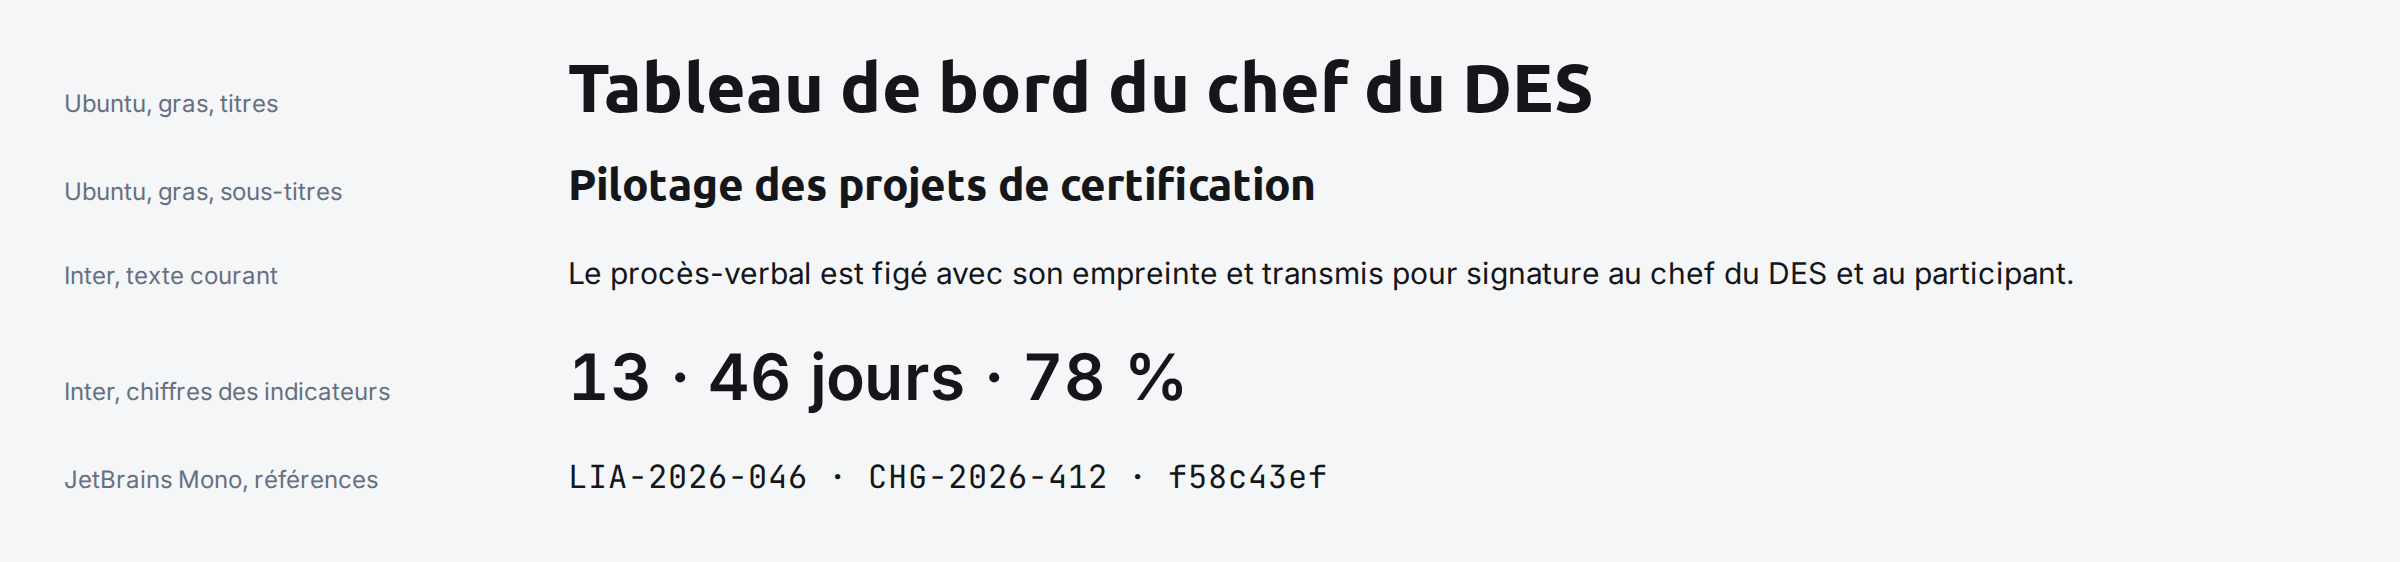
\includegraphics[width=0.97\linewidth]{typographie.png}}\end{center}

\subsection{Motifs}
Trois motifs habillent la plateforme. Ils restent discrets pour ne jamais gêner la lecture.
\begin{itemize}[leftmargin=1.2cm,itemsep=2pt]
\item \textbf{la trame} (à gauche) : des losanges couleur terre, inspirés des tissages de la sous-région ; elle sert de fond aux zones vides et aux discussions ;
\item \textbf{les courbes de niveau} (au centre) : elles évoquent le relief de l'Afrique centrale et couvrent l'écran de connexion ;
\item \textbf{le guillochage} (à droite) : des lignes fines et régulières, comme sur les billets de banque ; il remplit les lettres du nom Moabi sur l'écran de connexion.
\end{itemize}
\begin{center}\setlength{\fboxsep}{0pt}\fcolorbox{gris!40}{white}{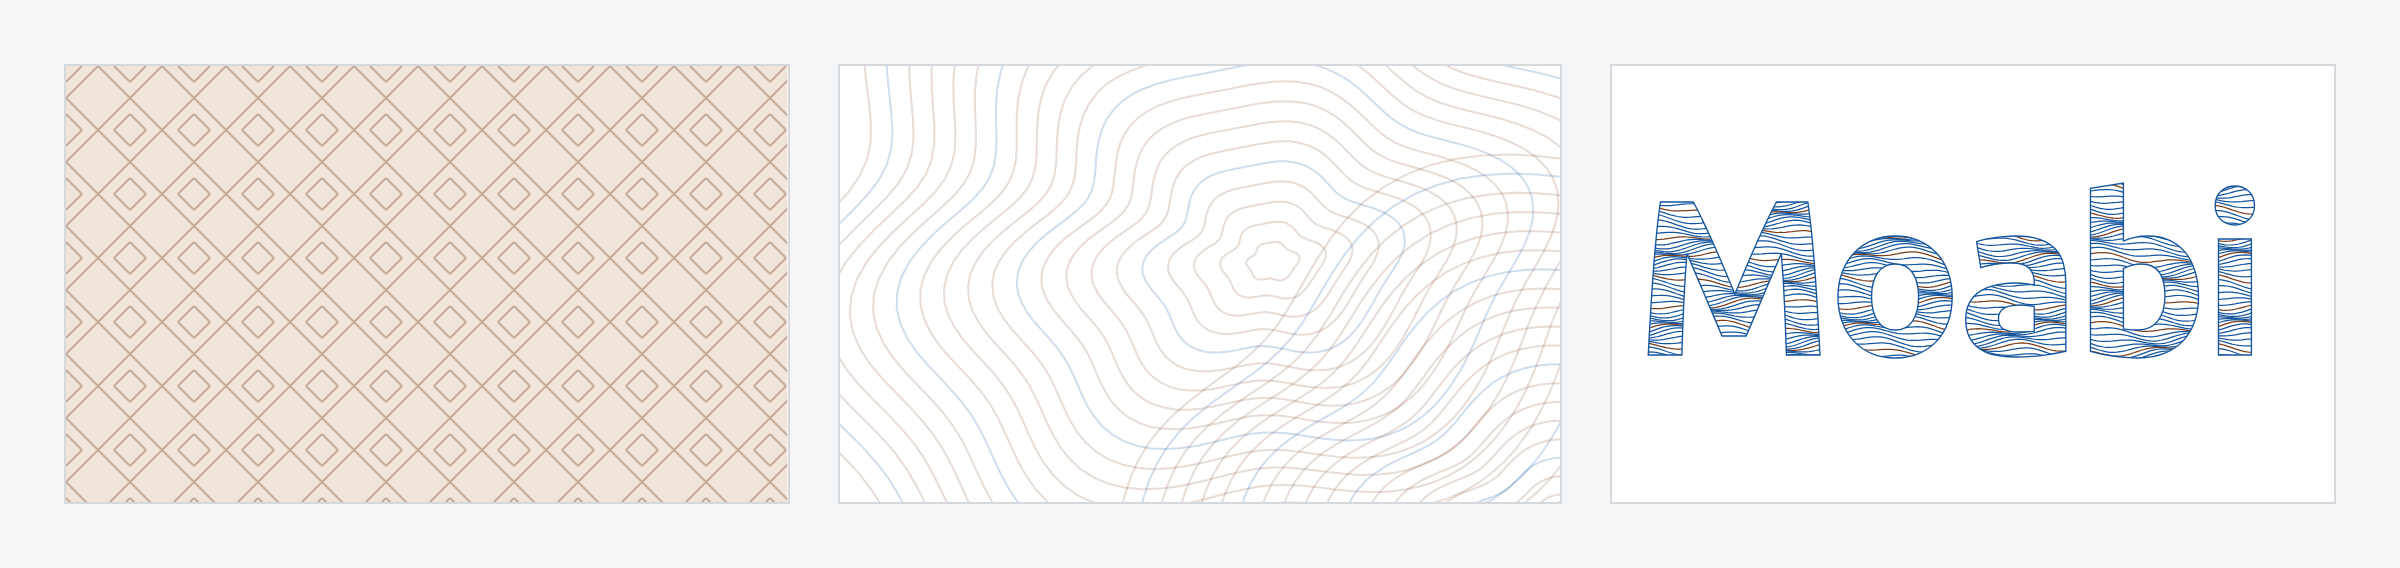
\includegraphics[width=0.97\linewidth]{motifs.png}}\end{center}

\subsection{Éléments d'interface}
Les boutons, les étiquettes d'état, les indicateurs et les champs de saisie sont les mêmes partout. Le bouton plein bleu marque l'action principale de l'écran. Le bouton encadré marque une action secondaire. Le lien simple sert à annuler. Le bouton rouge est réservé aux actions de refus. Les étiquettes de couleur donnent l'état d'un dossier d'un seul coup d'œil.

\begin{center}\setlength{\fboxsep}{0pt}\fcolorbox{gris!40}{white}{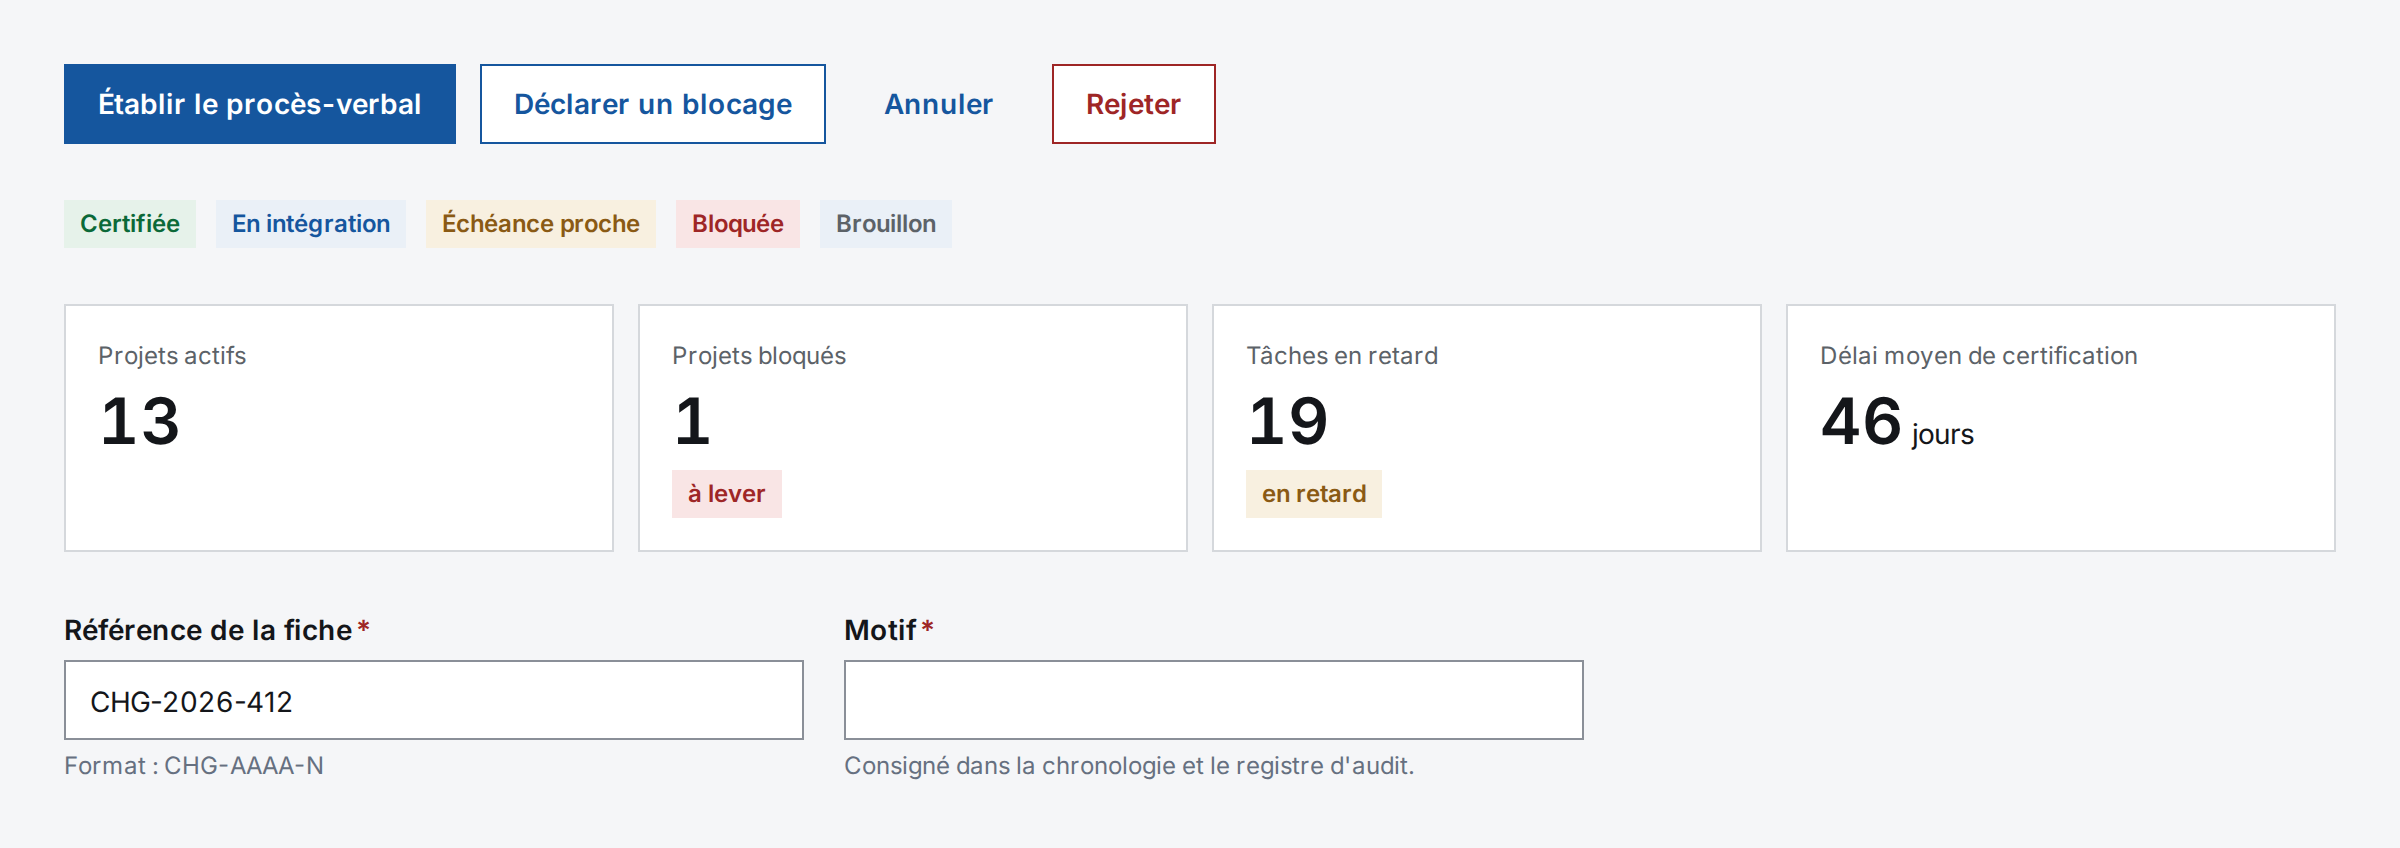
\includegraphics[width=0.97\linewidth]{composants.png}}\end{center}

\subsection{Mode clair et mode sombre}
Chaque utilisateur choisit son mode depuis le menu du globe, en haut à droite. En mode sombre, les fonds deviennent foncés, la barre latérale aussi, et les couleurs sont ajustées pour garder un bon contraste. Les éléments ci-dessous sont les mêmes que ceux de la section précédente, en mode sombre.

\begin{center}\setlength{\fboxsep}{0pt}\fcolorbox{gris!40}{white}{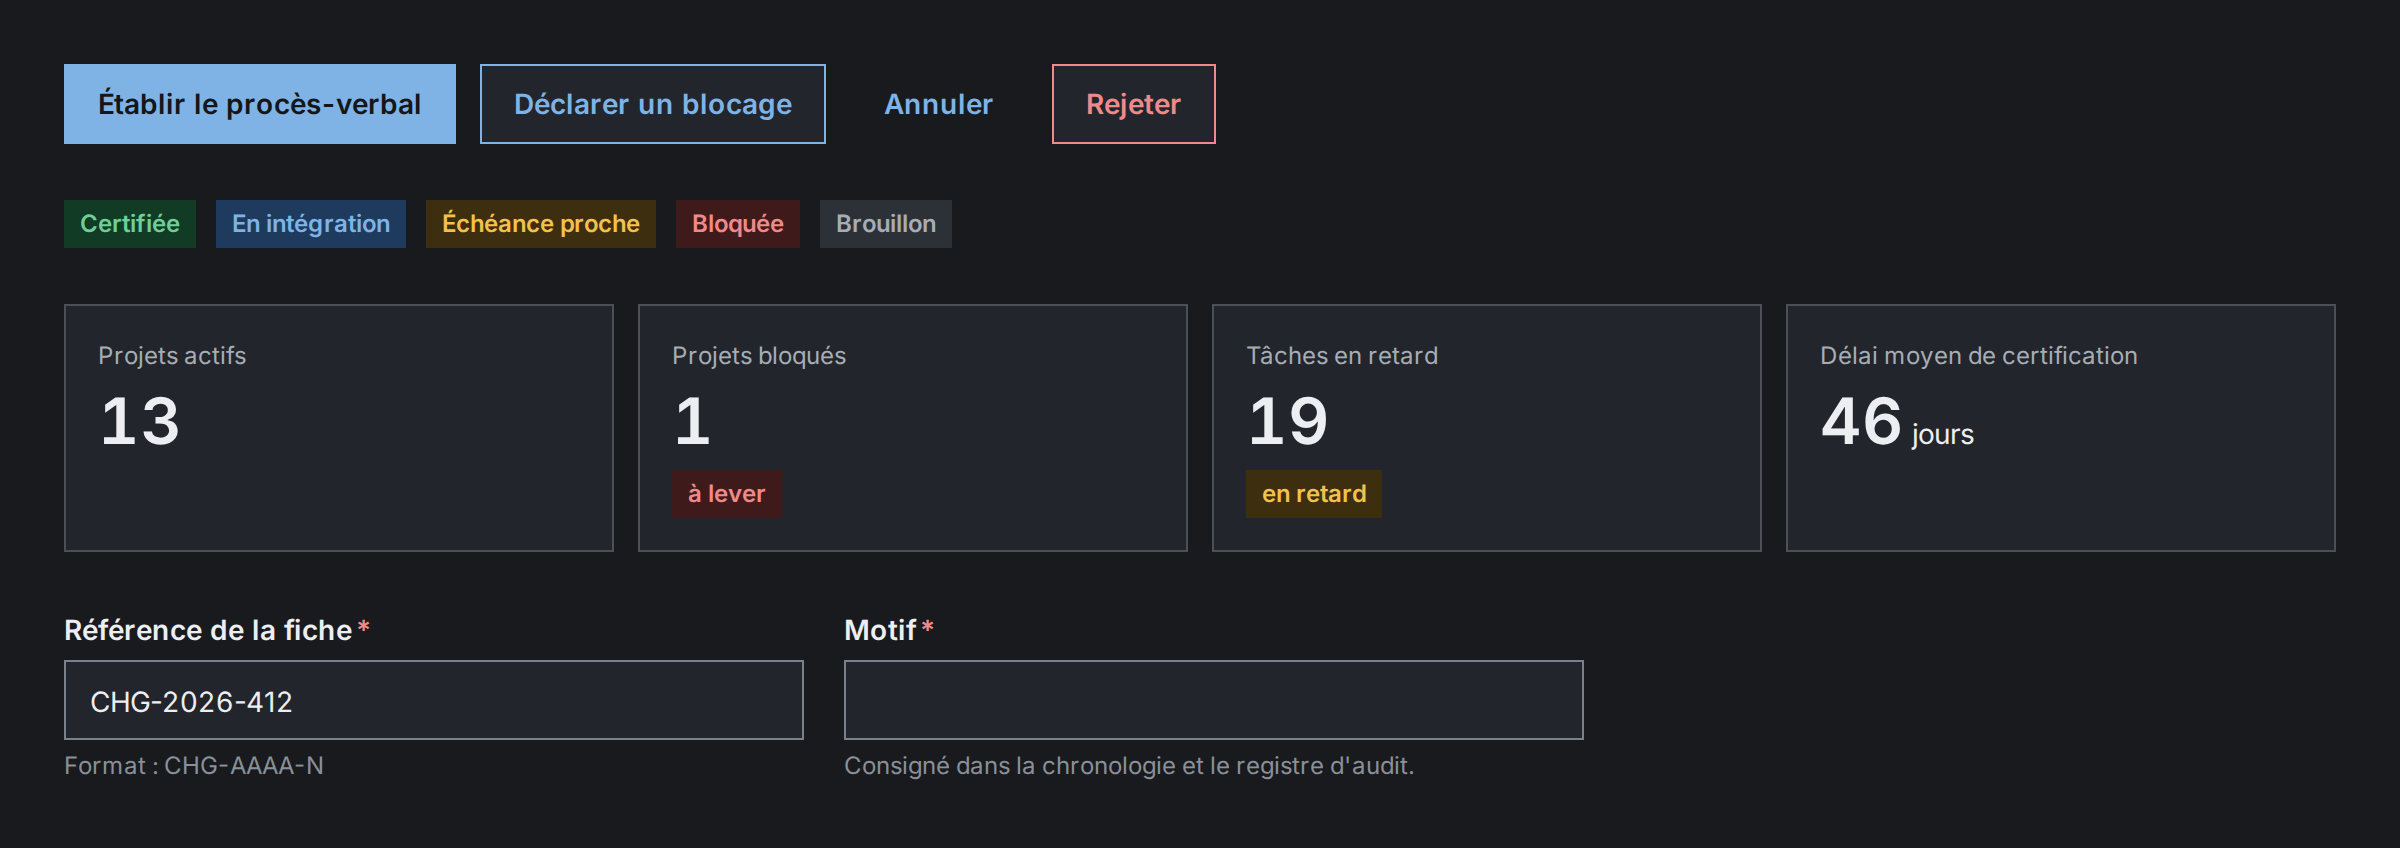
\includegraphics[width=0.97\linewidth]{composants-sombre.png}}\end{center}

\ecran{z01-connexion-sombre.jpg}{Écran de connexion en mode sombre}{En mode sombre, le nom Moabi est dessiné en contour. Les courbes de niveau restent visibles, plus discrètes.}
\ecran{z02-tdb-chef-des-sombre.jpg}{Tableau de bord en mode sombre}{Le tableau de bord du chef du DES en mode sombre. La barre latérale, les cartes et le graphique s'adaptent ; les couleurs d'état restent les mêmes.}
\ecran{z03-dossier-operations-sombre.jpg}{Dossier d'une liaison en mode sombre}{Le dossier numérique d'une liaison, onglet des opérations, en mode sombre.}
\ecran{z04-modale-sombre.jpg}{Fenêtre de dialogue en mode sombre}{Une fenêtre de dialogue en mode sombre : le fond de l'écran est voilé pour concentrer l'attention sur la saisie.}
\ecran{z05-tdb-portail-sombre.jpg}{Portail du participant en mode sombre}{Le portail des participants propose aussi le mode sombre.}

% ------------------------------------------------------------------ 4. Accès
\section{Accès à la plateforme}
La connexion se fait entièrement sur la plateforme. Il faut un identifiant, un mot de passe, puis un code à six chiffres donné par une application d'authentification sur téléphone. Une session sans activité pendant trente minutes se ferme d'elle-même.

\ecran{a01-connexion.jpg}{Écran de connexion}{C'est la première page que voit l'utilisateur. À gauche, la carte de connexion avec le logo du GIMAC, l'identifiant et le mot de passe. À droite, le nom de la plateforme. En haut à droite, le globe permet de changer de langue et la lune de passer en mode sombre. En bas, on lit l'application ouverte, la mention « usage interne, confidentiel » et l'heure de Douala avec l'heure universelle.}
\ecran{a02-code.jpg}{Saisie du code à six chiffres}{Après un mot de passe correct, la plateforme demande le code à six chiffres affiché par l'application d'authentification. Ce second contrôle protège le compte même si le mot de passe est connu d'une autre personne.}
\ecran{a03-oubli.jpg}{Mot de passe oublié}{L'utilisateur saisit son identifiant ou son adresse électronique. S'il a un compte actif, il reçoit un lien par courriel pour choisir un nouveau mot de passe. La réponse est toujours la même, pour ne pas révéler quels comptes existent.}
\ecran{a04-erreur.jpg}{Erreur de connexion}{En cas d'erreur, un message clair s'affiche en haut de la carte, avec un numéro de suivi. Ce numéro aide l'équipe technique à retrouver la cause si l'utilisateur la signale.}
\ecran{a05-premier-acces.jpg}{Premier accès}{À sa toute première connexion, l'utilisateur est guidé en quatre étapes : choisir son mot de passe, configurer son code à six chiffres, compléter ses coordonnées et accepter la charte d'utilisation. Tant que ces étapes ne sont pas faites, aucun autre écran n'est accessible.}

% ------------------------------------------------------------------ 5. DDRM
\section{Phase amont : prise de contact et adhésion (DDRM)}
La Direction du Développement et des Relations avec les Membres (DDRM) accueille les institutions candidates, instruit leur adhésion et prépare le lancement du projet.

\ecran{b01-tdb-chef-ddrm.jpg}{Tableau de bord du chef de la DDRM}{Le chef de la DDRM voit en haut les chiffres clés de sa direction : propositions à trancher, candidats, pièces à examiner, adhérents sans liaison. Plus bas figurent ses dossiers en cours et le pilotage d'ensemble des projets de certification. Chaque chiffre est un lien vers la liste concernée.}
\ecran{b02-institutions.jpg}{Institutions membres}{La liste de toutes les institutions, candidates ou membres, avec leur catégorie, leur pays et leur statut. Des filtres permettent de retrouver rapidement une institution. Le bouton en haut à droite enregistre une nouvelle prise de contact.}
\ecran{b03-fiche-institution.jpg}{Fiche d'une institution}{La fiche réunit tout ce qui concerne une institution : son identité, son dossier d'adhésion, les conditions d'adhésion, les prérequis et ses liaisons. Le bandeau indique où elle en est : candidat, adhérent, en homologation, actif.}
\ecran{b04-proposer-adhesion.jpg}{Proposer l'adhésion}{Quand le dossier est complet, la DDRM propose l'adhésion au chef de la DDRM. Un motif est demandé : il est conservé dans l'historique du dossier. Le chef de la DDRM approuve ensuite avec sa clé de sécurité.}
\ecran{b05-liaisons-amont.jpg}{Liaisons en phase amont}{La liste des liaisons encore au cadrage, au lancement ou aux ateliers. Pour chacune, on voit l'institution, l'étape, les tâches en retard, le conducteur de projet et les échéances.}
\ecran{b06-etapes.jpg}{Étapes d'une liaison}{Le parcours d'une liaison compte dix étapes. Ce tableau donne pour chacune son état (close, en cours, à venir), la fonction qui la porte, le nombre d'éléments réunis et l'échéance.}
\ecran{b07-depot-compte-rendu.jpg}{Dépôt d'un compte rendu d'atelier}{La DDRM dépose le compte rendu d'un atelier. La fenêtre rappelle l'opération concernée et le livrable attendu. Le fichier est glissé dans la zone prévue ; un commentaire peut l'accompagner.}
\ecran{b08-tdb-chargee-ddrm.jpg}{Tableau de bord de la chargée de la DDRM}{La chargée de la DDRM voit ses compteurs, ses dossiers en cours et la liste de ses tâches, avec leur échéance et leur niveau d'urgence.}
\ecran{b09-tiroir-operation.jpg}{Panneau d'une opération}{Chaque tâche ouvre un panneau latéral qui décrit l'opération : responsable, échéance, preuve attendue. C'est là que l'on dépose la preuve demandée, sans quitter le dossier.}
\ecran{b10-tiroir-intervenants.jpg}{Intervenants d'une opération}{L'onglet « Intervenants » du même panneau indique qui fait quoi sur l'opération : le responsable, le validateur, les personnes consultées et informées.}

% ------------------------------------------------------------------ 6. Chef du DES
\section{Pilotage par le chef du DES}
Le chef du DES ouvre les liaisons, désigne les conducteurs de projet, affecte les ressources et suit l'avancement de tous les projets.

\ecran{c01-tdb-chef-des.jpg}{Tableau de bord du chef du DES}{Le chef du DES suit l'ensemble des projets : projets actifs, projets bloqués, tâches en retard, échéances proches. Le graphique montre combien de projets se trouvent à chaque étape. À côté figurent le délai moyen de certification et le taux de respect des délais. Plus bas, six questions de pilotage reçoivent une réponse chiffrée.}
\ecran{c02-ouvrir-liaison.jpg}{Ouvrir une liaison}{Pour ouvrir une liaison, le chef du DES choisit l'institution adhérente, le type de projet, la banque partenaire éventuelle et le conducteur de projet. La liaison démarre alors à l'étape du cadrage.}
\ecran{c03-ouvrir-liaison-erreurs.jpg}{Contrôle de la saisie}{Si un choix manque, chaque champ concerné est signalé en rouge avec une explication. Rien n'est enregistré tant que la saisie n'est pas complète.}
\ecran{c04-designer-conducteur.jpg}{Désigner le conducteur de projet}{Le conducteur de projet suit la liaison jusqu'au suivi après production et établit le procès-verbal de certification. Le chef du DES le choisit dans la liste des personnes habilitées.}
\ecran{c05-liste-liaisons.jpg}{Liste des liaisons}{Toutes les liaisons, avec leur institution, leur étape, leurs alertes, leur conducteur, leur taux de certification et de mise en service, et leurs échéances. Les filtres se combinent et la vue peut être enregistrée pour être retrouvée plus tard.}
\ecran{c06-dossier-perimetre.jpg}{Dossier d'une liaison : périmètre}{Le dossier numérique réunit tout ce qui concerne une liaison. En haut : son identification et son pilotage. Le premier onglet montre la couverture des services du périmètre : ici, tous les services sont certifiés.}
\ecran{c07-dossier-etapes.jpg}{Dossier d'une liaison : étapes}{L'onglet « Étapes » reprend les dix étapes du parcours avec leur état et leur échéance. Un clic sur une étape en affiche le détail.}
\ecran{c08-dossier-operations.jpg}{Dossier d'une liaison : opérations}{L'onglet « Opérations » liste toutes les opérations de la liaison, regroupées par étape. Les compteurs indiquent ce qui reste à faire, à valider ou en retard. Une alerte attire l'attention sur une opération facile à oublier.}
\ecran{c09-dossier-decision.jpg}{Dossier d'une liaison : décision}{L'onglet « Décision » montre les verrous à franchir avant la mise en production : le procès-verbal de certification, puis l'approbation de la sécurité. Chaque verrou indique ce qui est fait et ce qui manque.}
\ecran{c10-dossier-mise-en-service.jpg}{Dossier d'une liaison : mise en service}{Après la mise en production, la fiche de suivi des services est remise au participant. Il y indique les services réellement ouverts ; Normes et Agréments le constate ensuite.}
\ecran{c11-dossier-blocages.jpg}{Dossier d'une liaison : blocages}{Les blocages en cours, avec le motif, l'étape, la date de début, la prochaine action, le responsable de la levée et l'échéance. Le bouton « Lever le blocage » le clôt lorsque le problème est réglé.}
\ecran{c12-dossier-gouvernance.jpg}{Dossier d'une liaison : gouvernance}{Les interlocuteurs du projet, côté GIMAC, côté participant et côté tiers. Chacun sait ainsi à qui s'adresser.}
\ecran{c13-declarer-blocage.jpg}{Déclarer un blocage}{Tout acteur concerné peut signaler un blocage. Il en donne le motif, la prochaine action, la fonction et la personne chargées de le lever, ainsi qu'une échéance. Le blocage reste visible de tous jusqu'à sa levée.}
\ecran{c14-etape-lancement.jpg}{Étape de lancement}{Le détail d'une étape. Ici, le lancement attend l'affectation des ressources du projet avant la réunion de lancement.}
\ecran{c15-affecter-ressources.jpg}{Affecter les ressources}{Le chef du DES désigne une personne par fonction : responsable fonctionnel, responsable technique, pôle réseau, pôle système, production monétique, sécurité et exploitation. La fenêtre signale les fonctions encore vides.}
\ecran{c16-referentiels.jpg}{Référentiels d'opérations}{Chaque type de projet suit un référentiel d'opérations, qui fixe les opérations à mener, leur ordre et leurs preuves. Les versions sont conservées. Une nouvelle version passe par un brouillon, un contrôle puis une publication.}

% ------------------------------------------------------------------ 7. Conducteur
\section{Conduite du projet}
Le conducteur de projet fait avancer la liaison au quotidien. Il valide les preuves déposées et établit le procès-verbal de certification.

\ecran{d01-tdb-conducteur.jpg}{Tableau de bord du conducteur de projet}{Le conducteur voit ses projets, les procès-verbaux à établir, ses tâches et ses échéances. La rubrique « Mes projets » donne l'avancement de chacune de ses liaisons.}
\ecran{d02-pv-a-etablir.jpg}{Procès-verbal à établir}{Quand la couverture de certification atteint cent pour cent, le procès-verbal peut être établi. L'écran montre la couverture, service par service, et l'état de chaque verrou.}
\ecran{d03-pv-confirmation.jpg}{Établir le procès-verbal}{Une confirmation est demandée avant d'établir le procès-verbal. Une fois établi, il est figé avec son empreinte et transmis pour signature au chef du DES et au participant.}
\ecran{d04-ceremonie-cles.jpg}{Cérémonie de clés}{Certaines opérations demandent des informations précises. Pour la cérémonie de clés, on saisit la date, les trois porteurs et les codes de contrôle des composantes. Aucun secret n'est demandé : seuls les codes de contrôle sont conservés.}
\ecran{d05-confirmation-depot.jpg}{Confirmation avant dépôt}{Avant tout dépôt, la plateforme résume ce qui va être enregistré pour une dernière vérification.}
\ecran{d06-validation-signee.jpg}{Validation signée}{Les actes importants sont signés avec une clé de sécurité. La fenêtre rappelle l'objet et l'empreinte de ce qui est signé. La signature est conservée dans le registre d'audit.}
\ecran{d07-tiroir-qualites.jpg}{Attribuer une qualité}{Le conducteur peut attribuer une qualité, par exemple celle de validateur, à un intervenant d'une opération. Le motif de ce choix est enregistré.}

% ------------------------------------------------------------------ 8. Pôles et SNA
\section{Pôles techniques et Normes et Agréments}
Les pôles réseau et système réalisent les travaux techniques. Normes et Agréments mène les essais, constate la couverture et la mise en service.

\ecran{e01-tdb-pole-reseau.jpg}{Tableau de bord du pôle réseau}{Le pôle réseau voit ses compteurs, comme les liens d'essai à établir, ses tâches et les liaisons qu'il suit.}
\ecran{e02-depot-preuve.jpg}{Dépôt d'une preuve}{Le pôle dépose la preuve de son travail, ici le contrôle d'atteignabilité du port. La preuve attend ensuite la validation du conducteur de projet.}
\ecran{e03-coordonnees-participant.jpg}{Coordonnées communiquées par le participant}{Les informations données par le participant depuis son portail, comme l'adresse et le port d'essai, se relisent directement dans l'opération.}
\ecran{f01-tdb-sna.jpg}{Tableau de bord de Normes et Agréments}{Normes et Agréments voit les essais en cours, les couvertures à constater, les mises en service à constater et ses tâches.}
\ecran{f02-constat-couverture.jpg}{Constat de la couverture}{La couverture est calculée par la plateforme à partir des essais. Normes et Agréments la constate. Tant qu'un service n'est pas concluant, le procès-verbal ne peut pas être établi.}
\ecran{f03-essais-simulateur.jpg}{Essais repris du simulateur}{Les résultats des essais sont repris du simulateur, service par service, sans nouveau calcul.}
\ecran{f04-remise-fiche.jpg}{Remise de la fiche de suivi}{Après la mise en production, Normes et Agréments remet la fiche de suivi des services au participant.}

% ------------------------------------------------------------------ 9. Décision
\section{Décision de mise en production}
La mise en production demande l'accord de plusieurs acteurs : la production monétique, la sécurité des systèmes d'information, la conformité et la direction générale.

\ecran{g01-tdb-production.jpg}{Tableau de bord de la production monétique}{La production monétique voit ses dossiers de changement, ses opérations à faire et ses tâches.}
\ecran{g02-fiche-changement.jpg}{Référencer la fiche de changement}{La production monétique indique la référence de la fiche de changement. La plateforme lit alors cette fiche dans l'outil de gestion des changements et en suit l'approbation.}
\ecran{h01-tdb-rssi.jpg}{Tableau de bord de la sécurité des SI}{Le responsable de la sécurité voit les attestations à vérifier et les approbations en attente.}
\ecran{h02-decision-attestations.jpg}{Vérification des attestations}{Le responsable de la sécurité examine les attestations fournies par le participant, par exemple PCI DSS. Il peut les déclarer conformes ou les rejeter, puis les archiver.}
\ecran{h03-rejet-attestation.jpg}{Rejet d'une attestation}{Le rejet demande un motif. Le participant le lit sur son portail et fournit une nouvelle attestation.}
\ecran{h04-tdb-conformite.jpg}{Tableau de bord de la conformité}{La conformité voit les visas attendus et les institutions suivies par la COBAC.}
\ecran{h05-visa-conformite.jpg}{Visa de la conformité}{La conformité donne son visa avec un motif et le signe avec sa clé de sécurité. Le visa est conservé dans le dossier.}
\ecran{h06-tdb-dg.jpg}{Tableau de bord de la direction générale}{La direction générale suit l'ensemble des projets de certification et donne son visa lorsqu'il est attendu.}

% ------------------------------------------------------------------ 10. Portail
\section{Portail du participant}
Le correspondant de l'institution utilise son propre portail. Il n'y voit que les liaisons de son institution.

\ecran{i01-tdb-portail.jpg}{Espace de certification du participant}{Le participant voit ce que le GIMAC attend de lui, avec l'échéance de chaque tâche. Un bouton mène directement à l'écran où il accomplit la tâche.}
\ecran{i02-mes-liaisons.jpg}{Mes liaisons}{Les liaisons de l'institution, avec l'étape en cours, le statut, les deux couvertures et la prochaine échéance.}
\ecran{i03-suivi-liaison.jpg}{Suivi d'une liaison}{Le participant suit son projet étape par étape. Il voit aussi les blocages qui le concernent, ses interlocuteurs au GIMAC et les pièces échangées.}
\ecran{i04-proces-verbal.jpg}{Procès-verbal de certification}{Le participant relit le procès-verbal : la couverture, les services certifiés, l'empreinte du document. Il le signe ensuite avec sa clé de sécurité.}
\ecran{i05-signature-cle.jpg}{Signature avec la clé de sécurité}{La signature se fait avec la clé de sécurité du correspondant. Elle est ensuite scellée dans le registre d'audit.}
\ecran{i06-coordonnees-essai.jpg}{Coordonnées d'essai}{Le participant communique l'adresse et le port de sa plateforme d'essai. La saisie est contrôlée avant l'envoi.}
\ecran{i07-fiche-suivi.jpg}{Fiche de suivi des services}{Après la mise en production, le participant indique pour chaque service s'il est réellement ouvert, avec un commentaire.}
\ecran{i08-attestations.jpg}{Attestations de sécurité}{Le participant consulte les attestations attendues et leur état de vérification par la sécurité du GIMAC.}

% ------------------------------------------------------------------ 11. Conclusion
\section{Conclusion}
Ce document a présenté les écrans du module de certification de la plateforme Moabi, de la connexion jusqu'au suivi après la mise en production, pour chacun des acteurs du parcours. Il a aussi présenté la charte graphique qui donne à l'ensemble une apparence cohérente, en mode clair comme en mode sombre.

Les remarques des collaborateurs sur ces écrans sont les bienvenues. Elles permettront d'ajuster les interfaces avant le chargement des données réelles et la mise en production du module.

\end{document}
